\newpage
\section{Tweaking the appearance and type of LANS output}
\label{sec:appearance}

\purplebox{}
Before you do any serious work with LANS, it is good to know that the appearance of the graphical output generated by LANS may \bb{not} be the same if produced by different versions of Matlab or if you use LANS on Windows, Linux or MacOS. This section describes how to resolve this issue. Note that you will need to deal with this issue only once, at the very beginning of working with LANS, as the system-specific settings will be stored on your computer when you close LANS and then reloaded when you start it the next time. 
\tcbe

\subsection{Adjusting the font size in the generated images and graphs}
\setcounter{step}{0}

\goldbox{}
The most prominent examples of where the differences occur include the appearance of the title and axis labels. Depending on the system and Matlab version, they can appear too large or too small relative to the size of the graph or image. Use the following steps to make the adjustments that suit your needs. 
\tcbe

\s{Select \lans{Preferences} $\ra$ \lans{Additional output options}.}

\s{In the new window that opens (Fig.~\ref{fig:appearance}), you will find several parameters in the  \lanstf{Magnification} \lanstf{printing factors} box. Adjust these factors individually for a~specific type of output, such as ion and ratio images, scatter plots, etc., and click \lans{Apply}.}

\sbx{Export an image or a graph (see below to learn how to do this) and check how it looks like.}

\s{You can also modify the font size by changing the value in the \lanstf{Fontsize of \dots} field.}

\nb{It is recommended that you experiment with the magnification factors a~little to get optimal results for your needs and taste.}

\nnb{If you reexport an image but the results do not seem to reflect the newly applied settings, you will need to close the image and export it again. This is because some features are only updated if the image is displayed anew.}

\begin{figure}[!t]
\centering
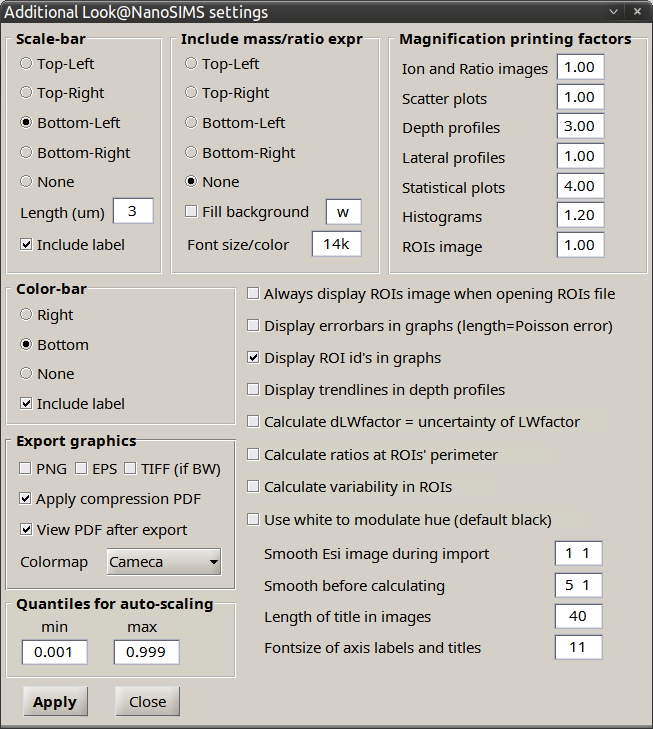
\includegraphics[scale=0.45]{figs1/LANS-tweaking}
\caption{\label{fig:appearance}%
Additional output options that can be tweaked in LANS.}
\end{figure}

\subsection{Further adjustments}
\label{sec:appearance1}

\goldbox{}
The \lans{Additional output options} window offers multiple other options for tweaking the appearance or type of output generated by LANS. Their thorough explanation goes beyond the scope of this document. Instead, you are encouraged to experiment and explore them by yourself. Here, we only highlight the ones that are most commonly used. Examples of the possible results are shown in Fig.~\ref{fig:appearance2}.
\tcbe

\nnb{\lanscb{\bb{Color bar}}: Color bar is relevant when displaying images of ion counts or ion count ratios. It can be placed below or to the right from the image. Relevant for this setting is the actual \lans{Colormap} (i.e., the correspondence between the value and color) in which the image is displayed. LANS offers numerous colormaps, which can be selected in the \lans{Export graphics} box.}

\nnb{\lanscb{\bb{Scale bar}}: Including a~scale bar is important when exporting images. You can specify its location within the image (top or bottom, left or right) and length (in $\mu$m). You can also specify whether the label of the scale bar, or the scale bar itself, should be included or not.}

\nnb{\bb{Title and annotation:} When working with mutliple datasets, it is useful if the generated output contains information that identifies the dataset and the variable displayed. In LANS, this information is included in the title and annotation of the graph or image. Whether or not the title should be included can be specified by checking the \lanscb{Graphs/image title} checkbox in the main LANS window, whereas settings in the \lanscb{Include mass/ratio expr} box in the \lans{Additional output options} window can be used to specify how to include additional annotatation.}

\nnb{\bb{Auto-scaling}: You can automatically set the scale of a~particular image by entering \ttt{[auto]} in the corresponding \lanstf{scale} field. The minimum and maximum of the scale is calculated, respectively, based on the \lanstf{min} and \lanstf{max} quantiles specified in the \lanscb{Quantiles for auto-scaling} box. }

\nnb{\bb{ROI annotation}: When displaying scatter plots, you can \lanscb{add ROI identification numbers} to each displayed data-point or \lanscb{include error-bars} indicating measurement precision (quantified by the Poisson error) by checking the corresponding checkboxes in the \lans{Additional output options} window.}

%%

\begin{figure}[!h]
\centering
\begin{tabular}{ccc}
A: 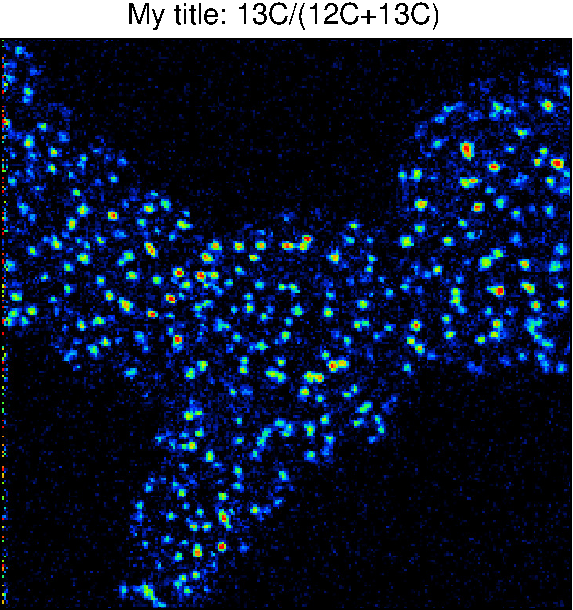
\includegraphics[scale=0.4, valign=t]{figs4/a-13C-(12C+13C)}
& 
B: 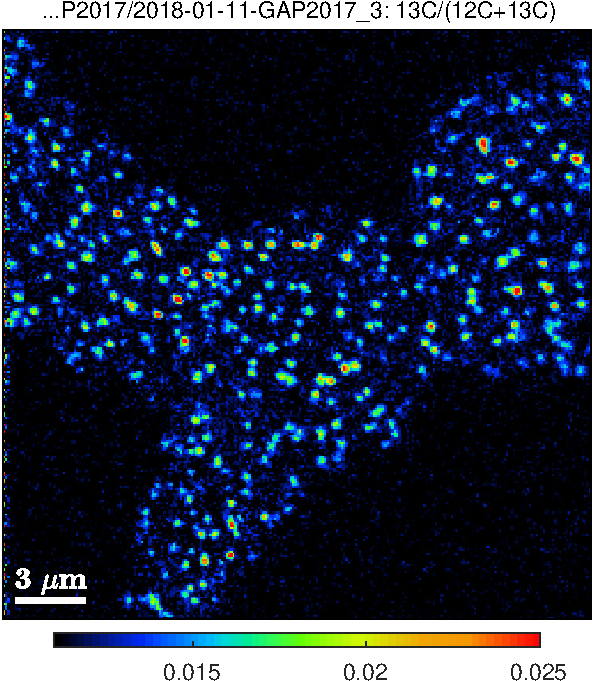
\includegraphics[scale=0.4, valign=t]{figs4/b-13C-(12C+13C)}
&
C: 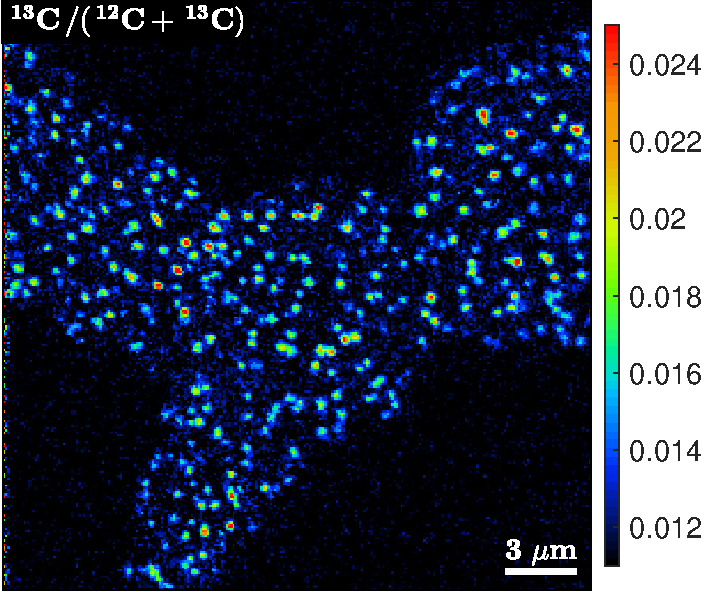
\includegraphics[scale=0.4, valign=t]{figs4/c-13C-(12C+13C)}
\end{tabular}
\\[5mm]
\begin{tabular}{ccc}
D: 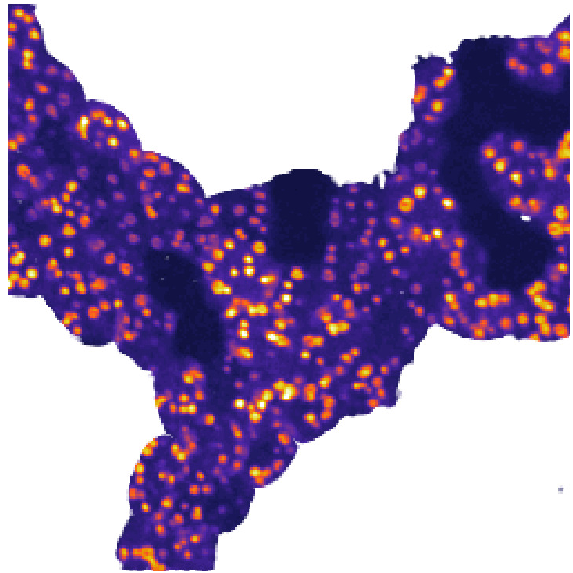
\includegraphics[scale=0.4, valign=t]{figs4/a-15N-14N}
& 
E: 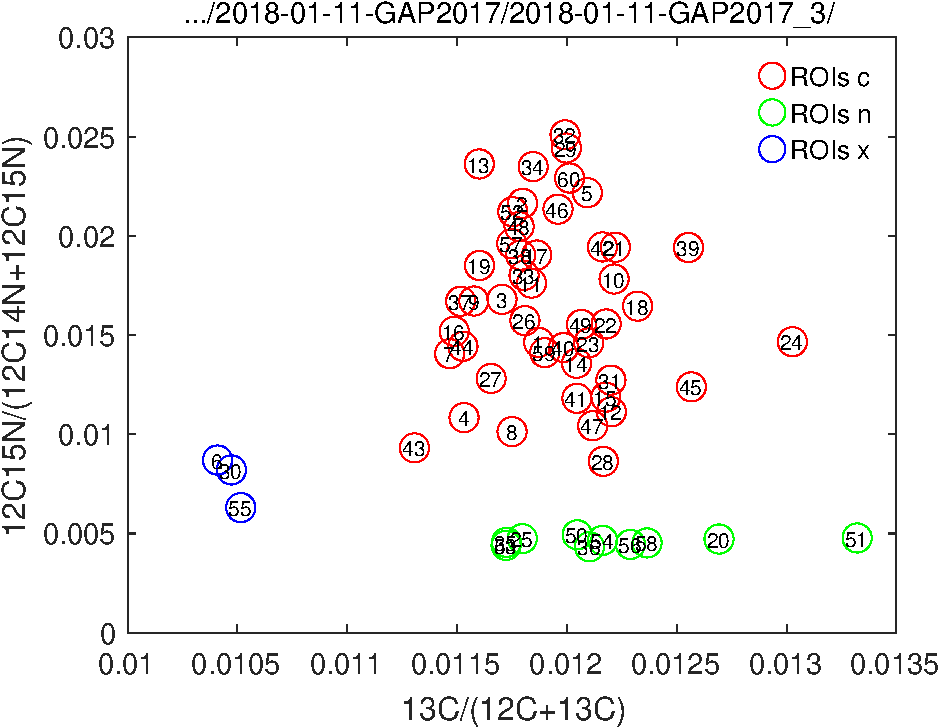
\includegraphics[scale=0.3, valign=t]{figs4/a-13C-15N}
&
F: 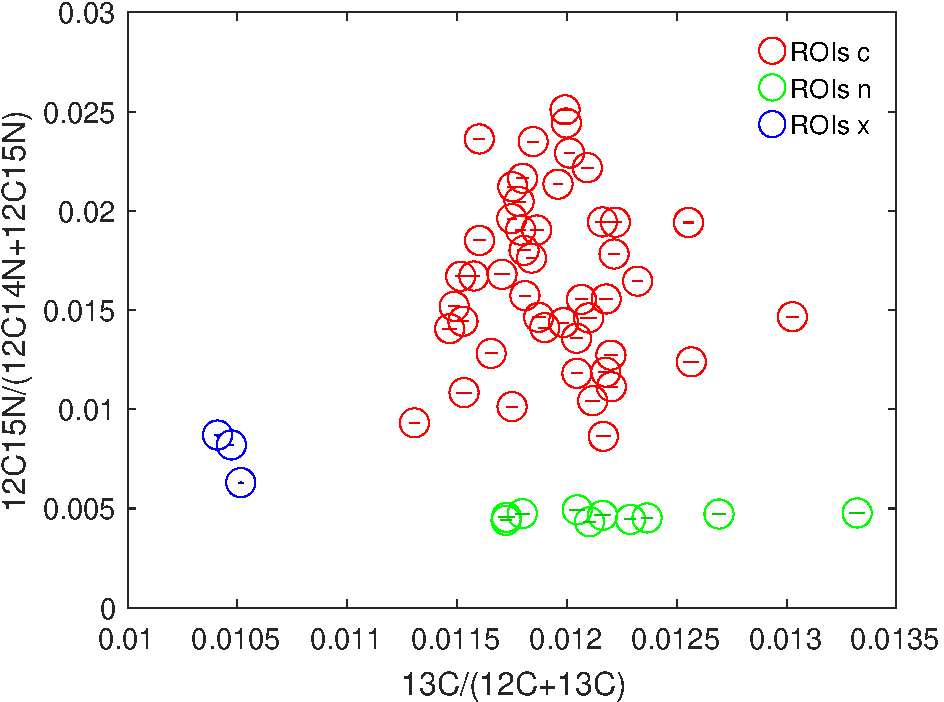
\includegraphics[scale=0.3, valign=t]{figs4/b-13C-15N}
\end{tabular}
\caption{\label{fig:appearance2}%
Examples of images and graphs generated by LANS. Panels A--C show different types of information and annotation that can be included in the images, including the title, color bar, scale bar, or formula of the displayed quantity. Panel D shows an image displayed in a~different colormap, without any annotation. Panels E and F show scatter plots with ROI identifiers and error-bars included, respectively.}
\end{figure}
